%************************************************
\chapter{Andamento do projeto}\label{ch:introducao}
%************************************************
\section{Sumário do projeto inicial}
Neste projeto, propomos o desenvolvimento de um método de reconhecimento de enovelamentos proteicos utilizando autômatos celulares. O reconhecimento do enovelamento é uma etapa crucial para expandir a utilização da modelagem comparativa, pois permite identificar proteínas que tenham estruturas semelhantes, mesmo na ausência de alta similaridade entre suas estruturas primárias. Além do reconhecimento do enovelamento proteico, os autômatos celulares apresentam características que os tornam capazes de fornecer também informações sobre a dinâmica do enovelamento, sendo, portanto, um método promissor nesta área, mas até então inédito.

Autômatos celulares são modelos computacionais que consistem num conjunto de células discretas espacialmente, as quais encontram-se em estado discreto num tempo também discreto. O estado dessas células podem se alterar ao longo do tempo para outros estados discretos pertencentes à um conjunto finito de estados possíveis. A alteração dos estados ao longo do tempo é chamada de evolução, e é definida por regras de transição simples e locais, onde o estado atual da célula e de seus vizinhos definirá para qual estado a célula irá evoluir. Esta evolução, muitas vezes, produz padrões complexos a partir do efeito cooperativo desses elementos simples - as regras e as células. Essa complexidade que surge globalmente  no sistema a partir de regras simples, locais e determinísticas é conhecida como Emergência.

A figura \ref{fig:ca} exemplifica um autômato celular elementar.
 

\begin{figure}[h]
	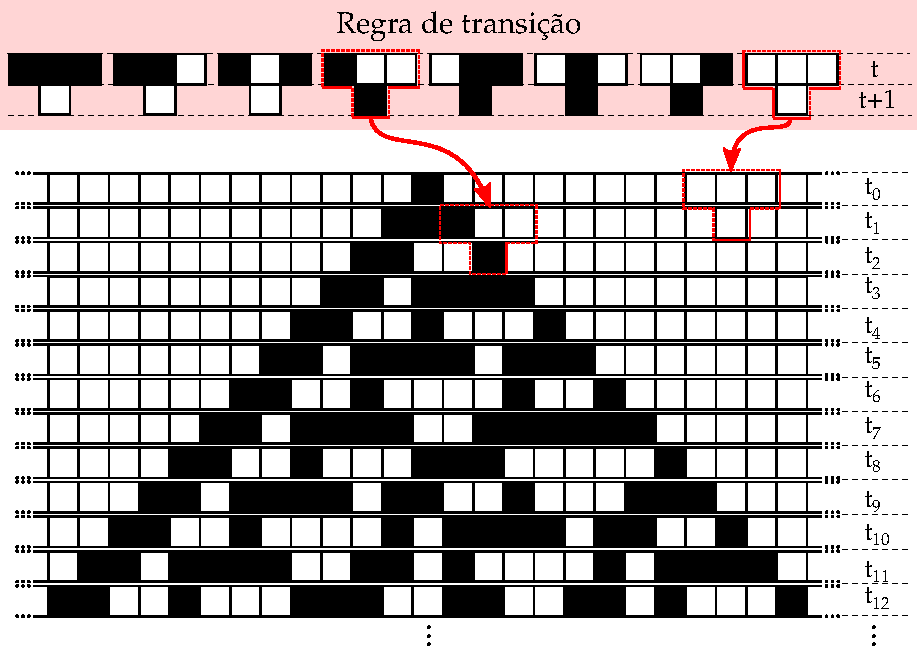
\includegraphics[width=1\linewidth]{ca_final}
	\caption{Exemplo de um autômato celular elementar. Este é o tipo de autômato celular mais simples, pois é unidimensional, possui apenas dois estados (0 ou 1) e possui vizinhança 1 (uma célula a esquerda e uma a direita). O autômato inicia com uma linha de células ($t_{0}$) e evolui através da aplicação de uma regra de transição que irá determinar o estado de cada uma das células na geração seguinte ($t_{1}$). Este processo ocorre iterativamente produzindo, muitas vezes, uma complexidade global que emerge da aplicação da regra local.}
	\label{fig:ca}
\end{figure}


\section{Análise do período}
Neste período, o código fonte inicial foi quase totalmente refeito para permitir maior flexibilidade. Isso foi necessário pois o código desenvolvido inicialmente e que foi utilizado em testes preliminares, abrangia apenas a predição da estruturas secundárias das proteínas e tinha como objetivo avaliar a viabilidade do projeto. 

As modificações feitas no código permitirá criar autômatos celulares com outros estados além dos já utilizados, que correspondam aos aminoácidos e a elementos de estrutura secundária. Portanto, isso possibilitará testarmos tanto códigos simplificados que representem, por exemplo, as características físico-químicas dos aminoácidos, como carga, polaridade, entre outros, assim como códigos mais complexos que representem, por exemplo, diversos elementos de estrutura secundária juntamente com a exposição ao solvente.

As disciplinas cursadas no período como  



Com a modificação dos objetivos do projeto para a criação de um método de reconhecimento de enovelamentos proteicos
\section{Discussões e conclusões parciais}
Discussões 
\section{Perspectivas futuras}
No próximo periodo
